\documentclass[twocolumn,amsfont,amssymb,amsmath, showpacs,balancelastpage, nofootinbib]{revtex4-1}
\pdfoutput=1

\usepackage{graphicx}
\usepackage{dcolumn}
\usepackage{bm}
\usepackage{amssymb,amsmath,bm}  
\usepackage{color}
\usepackage[colorlinks,linkcolor=red,citecolor=blue,urlcolor=blue ]{hyperref}
\usepackage{multirow}
\usepackage[utf8]{inputenc}
\usepackage{balance}
\usepackage{enumitem}
\usepackage{lipsum}
\newcommand{\nv}{\hat{\bf n}}
\newcommand{\kalo}{Karhunen-Lo\`{e}ve}

\begin{document}
\title{Science-driven 3D data compression}
\author{David Alonso$^1$}
\affiliation{$^{1}$Oxford Astrophysics, Department of Physics, Keble Road, Oxford, OX1 3RH, UK}

\begin{abstract}
  Photometric redshift surveys map the distribution of matter in the universe through the positions and shapes of galaxies with poorly resolved measurements of their radial positions. While a tomographic analysis can be used to recover some of the large-scale radial modes present in the data, this approach suffers from a number of practical shortcomings, and the criteria to decide on a particular binning scheme are commonly blind to the ultimate science goals. We present a method designed to separate and compress the data into a small number of uncorrelated radial modes, circumventing the main problems of standard tomographic analyses. The method is based on the \kalo transform, and is connected to other 3D data compression bases advocated in the literature, such as the Fourier-Bessel or Fourier-Laguerre bases. We apply this method to the specific cases of constraining dark energy with weak lensing and primordial non-Gaussianity with galaxy clustering. In the case of weak lensing we show that the method is able to compress the vast majority of the information into a single mode, considerably simplifying the analysis with respect to a traditional tomographic approach. \lipsum[0]
\end{abstract}

\maketitle

\section{Introduction}\label{sec:intro}
\lipsum[1]

\section{Method}\label{sec:method}
  \subsection{The Karhunen-Loeve transform}\label{ssec:method.klbasis}
    The idea behind the \kalo transform, as developed within the field of cosmological data analysis in e.g. CITES, is to compress a given data vector into a small set of modes containing most of the useful information on a particular parameter (or set of parameters). Let ${\bf a}$ be a data vector of dimension $N_s$, and let $\theta$ be a particular parameter we want to measure. Under the assumption that ${\bf x}$ is Gaussianly distributed with mean 0 and covariance ${\sf X}$, a set of linear combinations $y_p\equiv{\bf e}_p^\dag\,{\bf x}$ can be found such that the $y_p$ are white and uncorrelated ($\langle y_py_q^*\rangle=\delta_{pq}$) and such that the first $m<N_s$ combinations contain most of the information about $\theta$. This is done by solving the generalized eigenvalue problem CITE:
    \begin{equation}\label{eq:kl_general}
      \partial_\theta{\sf C}\,{\bf e}_p=\lambda_p\,{\sf C}\,{\bf e}_p,
    \end{equation}
    where $\partial_\theta\equiv\partial/\partial_\theta$.
    
    \subsubsection{The K-L transform for the signal-to-noise}\label{sssec:method.klbasis.sn}
      Let us decompose the data vector ${\bf x}$ into uncorrelated signal and noise components ${\bf x}={\bf s}+{\bf n}$ where, in this context, the signal is the part of the data containing any information of cosmological interest, and the noise is any contaminant preventing us to access it. In this particular case, the data covariance matrix can be split into their independent contributions ${\sf X}={\sf S}+{\sf N}$.
      
      The K-L transform has traditionally been used to design an eigenbasis that maximizes the overall signal-to-noise ratio (e.g. CITES). This can be done by defining a fictitious parameter $\alpha$ multiplying the signal part of the data with fiducial value $\alpha=1$ (i.e. ${\bf x}=\alpha{\bf s}+{\bf n}$). In this case, the eigenvalue equation (Eq. \ref{eq:kl_general}) takes the form:
      \begin{equation}\label{eq:kl_sn}
        ({\sf S}+{\sf N}){\bf e}_p=\lambda_p{\sf N}{\bf e}_p,
      \end{equation}
      where we have redefined $2/(2-\lambda_p)\rightarrow\lambda_p$. This can be cast into a standard eigenvalue equation using the Cholesky decomposition of the noise covariance matrix ${\sf N}={\sf L}{\sf L}^\dag$:
      \begin{equation}\label{eq:kl_sn_st}
        \left[{\sf L}^{-1}{\sf C}\,({\sf L}^{-1})^\dag\right]\,\tilde{\bf e}_p=\lambda_p\tilde{\bf e}_p,
      \end{equation}
      where $\tilde{\bf e}_p\equiv{\sf L}^\dag{\bf e}_p$.
      
      At this point it is worth noting that the generalized eigenvalue problem in Eq. \ref{eq:kl_sn} can be understood as the problem diagonalizing ${\sf C}$ under a non-standard dot product $\circ$ given by the inverse noise covariance matrix (i.e. ${\bf a}\circ{\bf b}\equiv{\bf a}^\dag{\sf N}^{-1}{\bf b}$. Under this dot product, an eigenbasis ${\sf F}\equiv({\bf f}_1,{\bf f}_2,...,{\bf f}_{N_s})$ can be found such that ${\sf F}$ is orthonormal ${\sf F}\circ{\sf F}={\sf I}$, and the covariance of the transformed data vector ${\bf y}\equiv{\sf F}\circ{\bf x}$ is diagonal:
      \begin{equation}\label{eq:kl_sn_prod}
        \langle{\bf y}\,{\bf y}^\dag\rangle={\sf F}^\dag{\sf N}^{-1}{\sf C}{\sf N}^{-1}{\sf F}={\sf \Lambda}\equiv{\rm diag}(\lambda_1,...,\lambda_{N_s}).
      \end{equation}
      Using the orthonormality of ${\sf F}$, this can be cast into the same form as Eq. \ref{eq:kl_sn_st}, where ${\bf f}_p={\sf L}\tilde{\bf e}_p={\sf N}{\bf e}_p$.
      
      Finally, note that, because both ${\sf S}$ and ${\sf N}$ are positive-definite matrices, their eigenvalues will also be positive. Since the eigenvalues of ${\sf N}$ under the K-L transform are, by construction, 1, the elements of $\Lambda$ above will all be greate than 1, and converging to 1 for the noise-dominated modes.
      
    \subsubsection{The K-L transform with correlated contaminants}\label{sssec:method.klbasis.cr}
      Let us now consider a more general case, where we further split the noise into two parts ${\bf n}\rightarrow{\bf n}+{\bf m}$, where ${\bf m}$ is a contaminant with a non-zero correlation with the signal. The covariance matrix of the data is then given by:
      \begin{equation}
        \langle{\bf x}\,{\bf x}^\dag\rangle=\alpha^2{\sf S}+2\alpha{\sf M}_s+{\sf M}+{\sf N},
      \end{equation}
      where ${\sf M}_s\equiv(\langle{\bf m}\,{\bf s}^\dag\rangle+\langle{\bf s}\,{\bf m}^\dag\rangle)/2$, ${\sf M}\equiv\langle{\bf m}\,{\bf m}^\dag\rangle$ and we have kept the fictitious parameter $\alpha$ defined in the previous section.
      
      Following the same steps as before, we obtain a similar generalized eigenvalue problem to that in Eq. \ref{eq:kl_sn}:
      \begin{equation}
        {\sf C}\,{\bf e}_p=\lambda_p\tilde{\sf N}\,{\bf e}_p
      \end{equation}
      with a modified noise covariance matrix $\tilde{\sf N}\equiv{\sf M}_s+{\sf M}+{\sf N}$. 

  \subsection{Application to tomographic datasets}\label{ssec:method.tomographic}
    The standard method to draw cosmological constraints from photometric redshift surveys is to divide the galaxy sample into bins in photo-$z$ space and use the information encoded in all the relevant auto- and cross-correlations between different bins, making use of various calibration methods in order to estimate the true redshift distribution of each bin. Several criteria can be followed in order to select these redshift bins, such as minimising the correlation between non-neighbouring bins or preserving a roughly constant number density on all bins. Other approaches (CITES) involve projecting the main observable (e.g. galaxy overdensity or shear) onto the Fourier-Bessel eigenbasis. None of these schemes are manifestly optimal from the point of view of $S/N$, final cosmological constraints or contaminant deprojection. This section presents an alternative slicing scheme addressing these shortcomings, based on the K-L transform.
    
    \subsubsection{Tomographic analyses}\label{sssec:method.tomographic.st}
      Let us start by assuming that we have split the galaxy sample into $N_s$ subsamples. As mentioned above, we will think of each of these subamples as some kind of redshift binning (e.g. binning galaxies in terms of their maximum-likelihood redshift), but the formalism applies to any set of subsamples. Let $f^\alpha(\nv)$ be the a field on the sphere at the angular position $\nv$ and defined in terms of the properties of the sources in the $\alpha$-th sample (e.g. the cosmic shear field $\gamma^\alpha$ or the galaxy overdensity $\delta^\alpha$), and let $\phi^\alpha(z)$ be the redshift distribution of these sources. Finally, let $a^\alpha_{\ell m}$ be the spherical harmonic coefficients of $f^\alpha$\footnote{Spin-2 fields, such as the cosmic shear, will be decomposed in spin-2 spherical harmonics, however the discussion below holds for fields of arbitrary spin.}. The power spectrum for our set of subsamples is defined as the two-point correlator of $a^\alpha$:
      \begin{equation}
        \left\langle {\bf a}_{\ell m}\,{\bf a}^\dag_{\ell' m'} \right\rangle\equiv\delta_{\ell\ell'}\delta_{mm'}{\sf C}_\ell,
      \end{equation}
      where we have packaged $a^\alpha$ as a vector for each $(\ell,m)$: ${\bf a}_{\ell m}\equiv(a^1_{\ell m},...,a^{N_s}_{\ell m})$. In general, the observed field will receive contributions from the true cosmological signal (${\bf s}$) and measurement noise (${\bf n}$).
  
      Once the choice of subsamples $\alpha$ is made, the standard analysis method would proceed by performing a likelihood evaluation of the two-point statistics of these subsamples. While this procedure is relatively simple, it suffers from a number of drawbacks, an incomplete list of which is:
      \begin{enumerate}
        \item It is not clear what the optimal strategy should be to define the sub-samples. One could make sure to exploit all of the information present in the data by using a large number of very narrow redshift bins, and let the likelihood evaluation pick up the information encoded in them.
        \item $C^{\alpha\beta}_\ell$ is a $N_s\times N_s\times N_\ell$ data vector. Thus increasing $N_s$ will increase the computational time required for each likelihood evaluation like $N_s^2$ and number of elements of the covariance matrix of $C^{\alpha\beta}_\ell$ like $N_s^4$, with the corresponding increase in complexity needed to estimate this covariance. Although this can be partially alleviated by considering only correlations between neighbouring redshift shells, the amount of information lost by neglecting all correlations beyond a given neighbouring index is not clear a priori.
        \item Estimating the redshift distribution for a large number of subsamples can be inaccurate, depending on the method used to do so, on the quality of the photometric redshift posterior information and on the statistics of the available spectroscopic sample.
     \end{enumerate}
  
    \subsubsection{Optimal radial eigenbasis}\label{sssec:method.tomographic.kl}
      Following the description in Section \ref{sssec:method.klbasis.sn}, it is straightforward to derive an optimal set of radial, uncorrelated eigenmodes.
      \begin{enumerate}
        \item We start by assuming that the field ${\bf a}$ has been measured in a number of narrow redshift bins, and by defining the inverse-variance weighted field $\tilde{\bf a}_{\ell m}\equiv{\sf N}^{-1}_\ell\,{\bf a}_{\ell m}$.
        \item Let us consider a set of linear combinations of the weighted field measured on narrow redshift bins:
        \begin{equation}
          {\bf b}_{\ell m}={\sf F}_\ell^\dag\cdot\tilde{\bf a}_{\ell m}\equiv{\sf F}_\ell\circ{\bf a},
        \end{equation}
        where ${\sf F}_\ell$ is a yet-unspecified matrix and, as in Section \ref{sssec:method.klbasis.sn}, we have let ${\sf N}^{-1}$ define the non-standard dot product ${\bf v}_\ell\circ{\bf w}_\ell\equiv{\bf v}^\dag_\ell\cdot{\sf N}^{-1}_\ell\cdot{\bf w}_\ell$. The power spectrum for this new observable would then simply be given by:
        \begin{equation}\label{eq:dp_uncouple}
          {\sf D}_\ell\equiv\left\langle{\bf b}_{\ell m}\,{\bf b}^\dag_{\ell m}\right\rangle={\sf F}_\ell^\dag\circ{\sf C}_\ell\circ{\sf F}_\ell.
        \end{equation}
        \item Requiring that the new modes be uncorrelated, we can identify Eq. \ref{eq:dp_uncouple} with the generalized eigenvalue equation \ref{eq:kl_sn_prod}, which defines the K-L eigenbasis ${\sf F}_\ell$ by additionally requiring that it be orthonormal (${\sf F}_\ell\circ{\sf F}_\ell={\sf I}$). Note that, after this transformation and without any further optimization, some of the practicalities of the original problem the original problem are already simplified, since we can now focus on the diagonal elements of the new power spectrum and its covariance.
        \item The data can be further compressed if by assuming that we are interested in measuring a set of cosmological parameters $\Theta\equiv\{\theta_1,...\}$. The information regarding this set of parameters encoded in a given data vector ${\bf x}$ can be quantified in terms of its Fisher matrix (the expectation value of the Hessian of the log-likelihood with respect to $\Theta$), which assuming $\langle{\bf x}\rangle=0$ reads
        \begin{equation}
          {\cal F}_{ij}\equiv\left\langle\partial_i\partial_j{\cal L}\right\rangle=\frac{1}{2}{\rm Tr}\left(\partial_i{\sf X}\,{\sf X}^{-1}\partial_j{\sf X}\,{\sf X}^{-1}\right),
        \end{equation}
        where ${\sf X}\equiv\langle {\bf x}\,{\bf x}^\dag\rangle$ is the covariance matrix of the data. Since the power spectrum of ${\bf b}_{\ell m}$ defined above is diagonal, this expression gets simplified further, and the Fisher matrix can be decomposed into the independent contributions of each mode: ${\cal F}_{ij}=\sum_p {\cal F}^p_{ij}$, where
        \begin{align}
          {\cal F}^p_{ij}&\equiv\sum_\ell\frac{2\ell+1}{2}\,(\partial_i\log D^p_\ell)\,(\partial_j\log D^p_\ell).
        \end{align}
        We can thus rank the eigenvectors $({\sf F}_\ell)^p_\alpha$ in terms of their information content (in a Fisher-matrix sense).
        \item The final set of uncorrelated modes can then be truncated to the first $M$ defined by this procedure, which will contain the bulk of the information needed to constrain $\Theta$.
    \end{enumerate}
    This strategy therefore allows one to reliably and significantly reduce the dimensionality of the data vector from $N_s^2\times N_\ell$ to $M\times N_\ell$ while minimising the loss of information. Note that, although the method is based on an initial thin-slicing of the galaxy distribution, the fact that the final datased comprises only a small set of samples means that the method is not penalized in terms of photometric redshift uncertainties. Once the K-L eigenmodes ${\sf F}_\ell$ are found for a fiducial cosmological model, they can be directly applied as weights to all the objects in the survey to generate the $b^p_\ell$ modes. Furthermore, using ${\sf F}_\ell$ for the fiducial cosmology as model-agnostic weights and inserting them in Eq. \ref{eq:dp_uncouple}, the theoretical prediction for the power spectrum of each mode $D^p_\ell$ can be computed in a model-independent way.
    
    The same methods used to calibrate photo-$z$ uncertainties in the standard tomographic analysis hold in this case with slight modifications (e.g. weighed and $\ell$-dependent stacking of photo-$z$ pdfs, or cross-correlations of the weighed maps with a spectroscopic survey in the case of clustering redshifts).


\section{Performance and particular examples}\label{sec:results}
  This Section explores the performance of the K-L decomposition in a number of specific science cases.
  
  \subsection{Special case: the harmonic-bessel basis}\label{ssec:results.bessel}
    Let us consider a simplified case where $f$ is the overdensity field of a non-evolving galaxy population for which we neglect the effect of redshift-space distortions. Let us further assume that we have perfect redshift information, such that we can split the sample into thin radial slices of equal width $\delta r$, which we label by their comoving radius $r$. The noise in the measurement of $f$ is given purely by shot noise, and since (as per our initial assumptions) the number density of sources does not change with $r$, the noise power spectrum is diagonal and scales like 
    \begin{equation}
      N_\ell(r,r')\propto \frac{\delta_{r,r'}}{r^2}.
    \end{equation}
    Thus, the dot product is just given by:
    \begin{equation}
      {\bf b}^\dag\circ{\bf c}\propto\int dr\,r^2\,b(r)^*\,c(r).
    \end{equation}
    \begin{figure*}
      \centering
      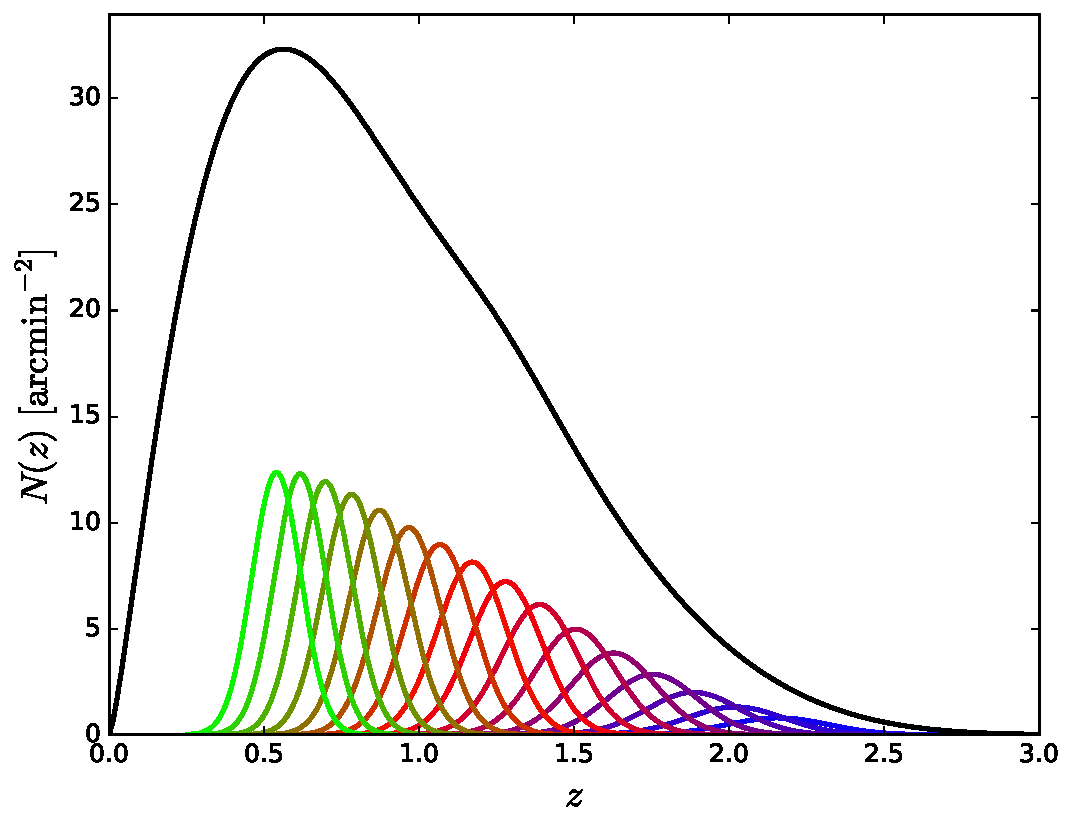
\includegraphics[width=0.49\textwidth]{Figs/nz_lsst_wl}
      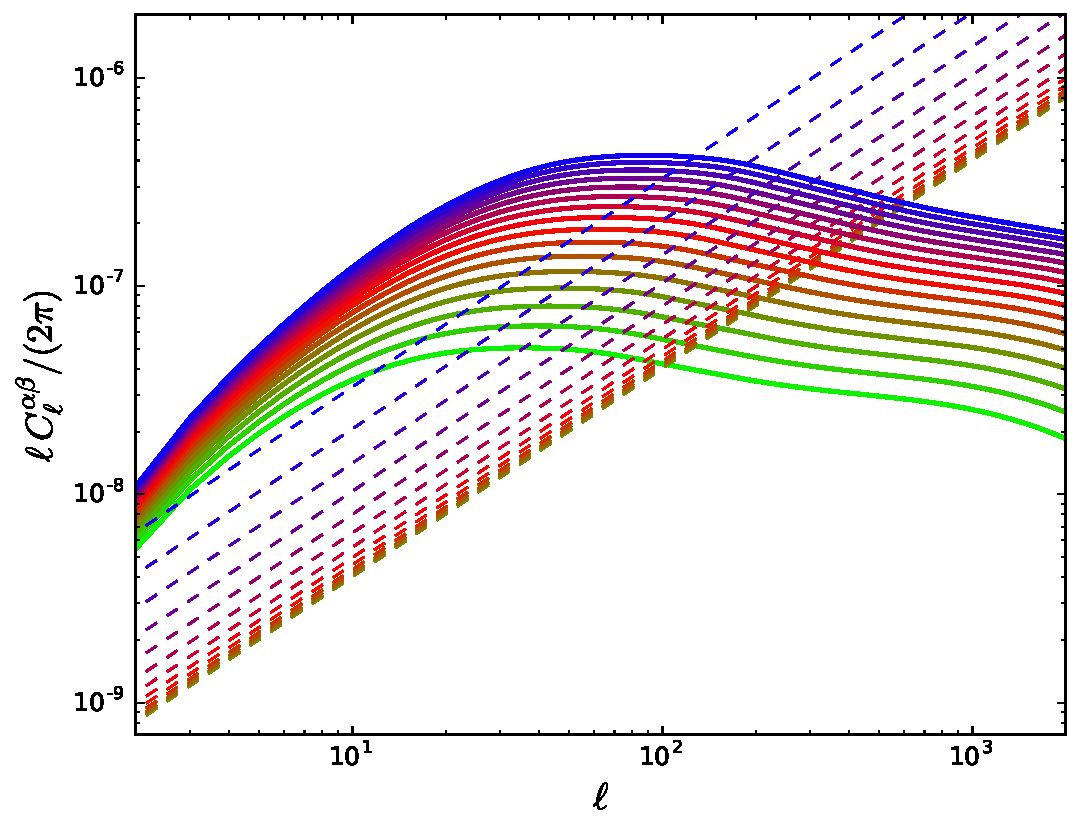
\includegraphics[width=0.49\textwidth]{Figs/c_ij_wl}
      \caption{{\sl Left}: redshift distribution and bins considered for the K-L analysis of a strawman weak-lensing survey. {\sl Right}: shear auto-power spectra of the redshift bins shown in the left panel. The signal and noise power spectra are shown as thick solid and thin dashed lines respectively.}\label{fig:nz_wl}
    \end{figure*}
   
    In this case, the cross-shell power spectrum is given by,
    \begin{equation}
      C_\ell^{rr'}=\frac{2}{\pi}\int_0^\infty dk\,k^2\,P_k\,j_\ell(kr)j_\ell(kr'),
    \end{equation}
    and it is trivial to show that the K-L eigenmodes are simply given by the spherical Bessel functions: $({\sf F}_\ell)^k_r\propto \sqrt{2/\pi}j_\ell(kr)$:
    \begin{widetext}
    \begin{align}
      D_\ell^{kk'}&\propto\frac{2}{\pi}\int dr\,r^2\int dr'\,r'^2 j_\ell(kr)j_\ell(k'r') C_\ell^{rr'}\\
      &=\int dq\,q^2P_q\left[\frac{2}{\pi}\int dr\,r^2\,j_\ell(qr)j_\ell(kr)\right]\left[\frac{2}{\pi}\int dr'\,r'^2\,j_\ell(qr')j_\ell(k'r')\right]\\
      &=\int dq\,q^2P_q\frac{\delta(k-q)}{q^2}\frac{\delta(k'-q)}{q^2}=P_k\frac{\delta(k-k')}{k^2}=\frac{P_k}{k^2\Delta k}\delta_{k,k'}
    \end{align}
    \end{widetext}
   
    This choice of basis defines the so-called harmonic-Bessel (or Fourier-Bessel) decomposition, and has been postulated as a possible data-compression method for the analysis of photometric redshift data (CITES here). In any realistic scenario however (e.g. in the presence of redshift uncertainties, RSDs or for the analysis of weak lensing data), this basis is non-optimal (e.g. different $k$s will be correlated), as opposed to the K-L basis described above.

  \subsection{Weak lensing - K-L basis for dark energy}\label{ssec:results.wl}
    \begin{figure}
      \centering
      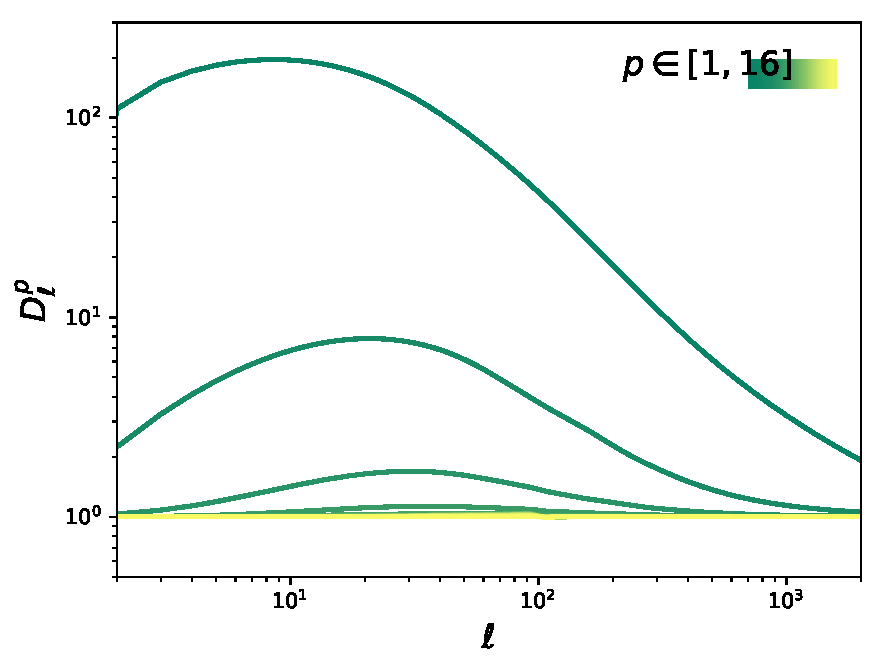
\includegraphics[width=0.49\textwidth]{Figs/d_p_wl}
      \caption{Power spectra of the K-L eigenmodes for the strawman weak lensing survey. All but the first three modes are noise-dominated, and most of the information is encoded in the first mode.}\label{fig:dp_wl}
    \end{figure}
    \begin{figure}
      \centering
      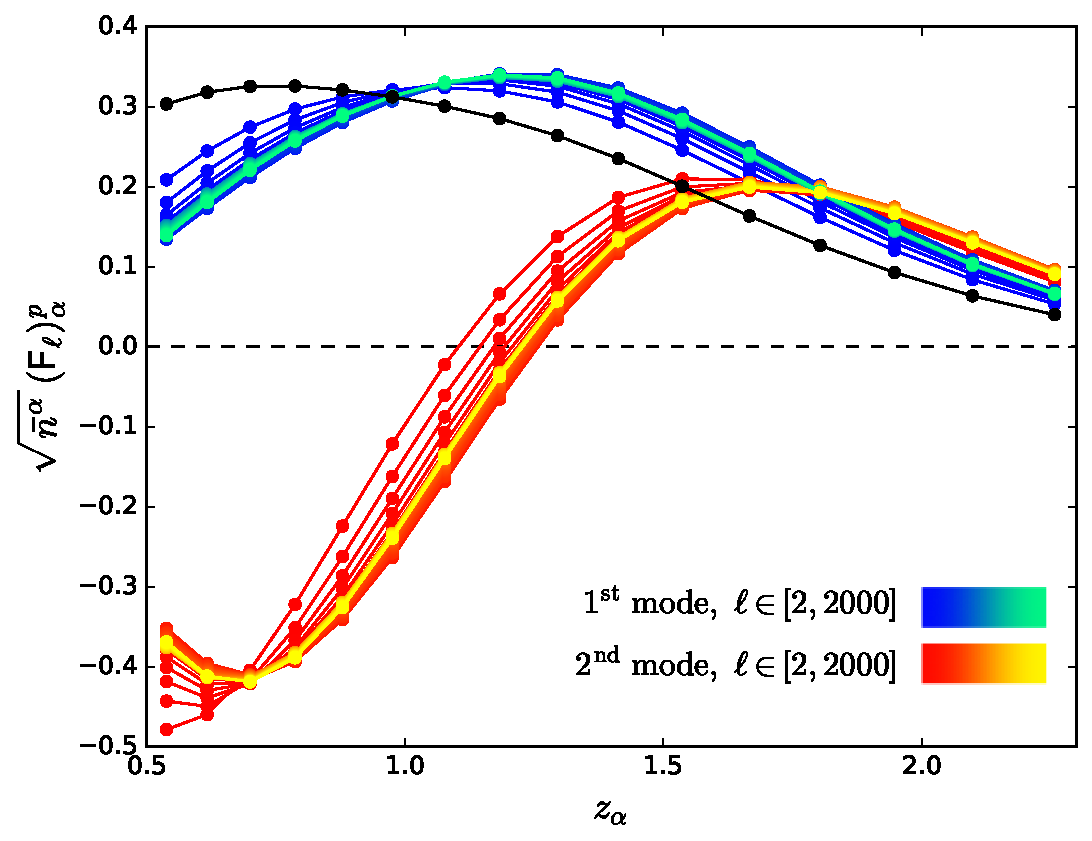
\includegraphics[width=0.49\textwidth]{Figs/kl_modes_wl}
      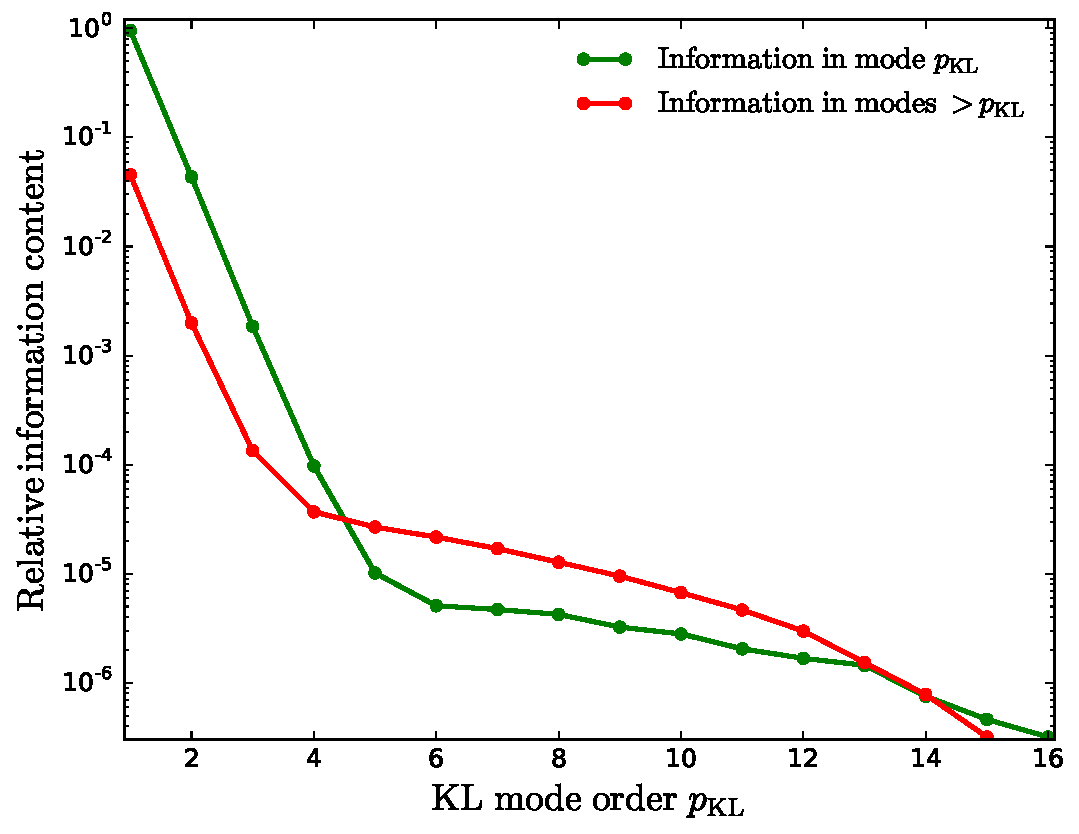
\includegraphics[width=0.49\textwidth]{Figs/information_wl}
      \caption{{\sl Left}: the first (blue-cyan) and second (red-yellow) eigenmodes of the strawman weak-lensing survey for different $\ell$. The redshift dependence of the modes stays roughly constant across $\ell$ and converges to a fixed shape for large $\ell$. {\sl Right}: information content of the different eigenmodes. Most of the information $\sim95\%$ is encoded in the first bin, and more than $99\%$ of it can be recovered considering only the first 2 modes.}\label{fig:kl_wl}
    \end{figure}
    To quantify the performance of the K-L modes for weak lensing we study the case of an LSST-like survey. The survey specifications and the characteristics of the galaxy sample are described in detail in CITE. In summary, we assume a sample with $\sim29$ objects per ${\rm arcmin}^2$ with the redshift distribution shown in the left panel of Figure \ref{fig:nz_wl}. We also approximate the photo-$z$ distribution as Gaussian with a scatter $\sigma_z=0.05\,(1+z)$.    
    
    The signal part of the cross-power spectrum between the cosmic shear measurements made in two different redshift shells is given by:
    \begin{equation}\label{eq:cl_generic}
      S^{\alpha\beta}_\ell=\frac{2}{\pi}\int_0^\infty dk\,k^2\,\Delta^\alpha_\ell(k)\Delta^\beta_\ell(k),
    \end{equation}
    where the transfer functions $\Delta^{\alpha}_\ell$ take the form:
    \begin{align}\nonumber
      &\Delta^{\gamma,\alpha}_\ell(k)\equiv\sqrt{\frac{(\ell+2)!}{(\ell-2)!}}\int d\chi\,W^\alpha(\chi)\frac{j_\ell(k\chi)}{k^2a(\chi)}\sqrt{P(k,z(\chi))},\\%\hspace{12pt}
      &W^\alpha(\chi)\equiv\frac{3H_0^2\Omega_M}{2}\int_{z(\chi)}^\infty dz\,\phi^\alpha(z')\frac{\chi(z')-\chi}{\chi(z')\chi}.
    \end{align}
    Here $\phi^\alpha(z)$ is the redshift distribution of sources in the $\alpha$-th bin. The noise power spectrum is white and simply given by the intrinsic ellipticity scatter weighed by the number density of sources in each redshift bin $\bar{n}^\alpha$:
    \begin{equation}
      N^{\alpha\beta}_\ell=\delta_{\alpha\beta}\frac{\sigma_\gamma^2}{\bar{n}^\alpha},
    \end{equation}
    with $\bar{n}^\alpha$ in units of ${\rm srad}^{-1}$. We use $\sigma_\gamma=0.28$.
    
    As our initial set of narrow redshift bins, we select top-hat bins in photo-$z$ space for $z_{\rm ph}>0.5$ with a width given by the value of $\sigma_z$ at the center of the bin. The resulting set of 16 bins is shown in the left panel of Figure \ref{fig:nz_wl}. The large overlap between bins implies that a choice of thinner slices is unlikely to unveil significantly more information, and we have verified that the results shown below do not change after doubling the number of bins. The lensing auto-power spectra (both signal and noise) for these bins are shown in the right panel of Figure \ref{fig:kl_wl}. The elements of $C^{\alpha\beta}_\ell$ were estimated using a modified version of the code presented in CITE.
    
    We compute the K-L modes for this setup and rank them according to their information content on the dark energy equation of state $w$. The power spectra of the resulting set of modes are shown in the left panel of Figure \ref{fig:dp_wl}. Comparing against the right panel of Fig. \ref{fig:nz_wl} we can see that the K-L decomposition effectively separates the signal-dominated and noise-dominated modes, with all modes $p>3$ dominated by noise (as we mentioned in Section \ref{sssec:method.klbasis.sn}, the noise power spectrum gets mapped into $1$ under the K-L transform). The fractional contribution of each mode to the total constraint on $w$ (i.e. its contribution to the corresponding Fisher matrix element) is shown in the left panel of Figure \ref{fig:kl_wl}. Most of the information ($\sim95\%$) is contained within a single mode, and the first two modes are able to recover more than $99\%$ of the total. The eigenvectors corresponding to the first and second modes for different values of $\ell$ are shown in the right panel of the same figure. Firstly, we observe that the eigenvectors preserve roughly the same shape for all $\ell$, and converge to the same shape at large $\ell$. The first eigenvector upweights the parts of the redshift range with the highest signal-to-noise, penalising the low-$z$ regime due to its poor lensing signal and the high-$z$ bins due to their high shot noise. The second eigenmode then recovers part of this information by marginally upweighting these regions.

  \subsection{Galaxy clustering - measuring $f_{\rm NL}$}\label{ssec:results.fnl}
    \begin{figure*}
      \centering
      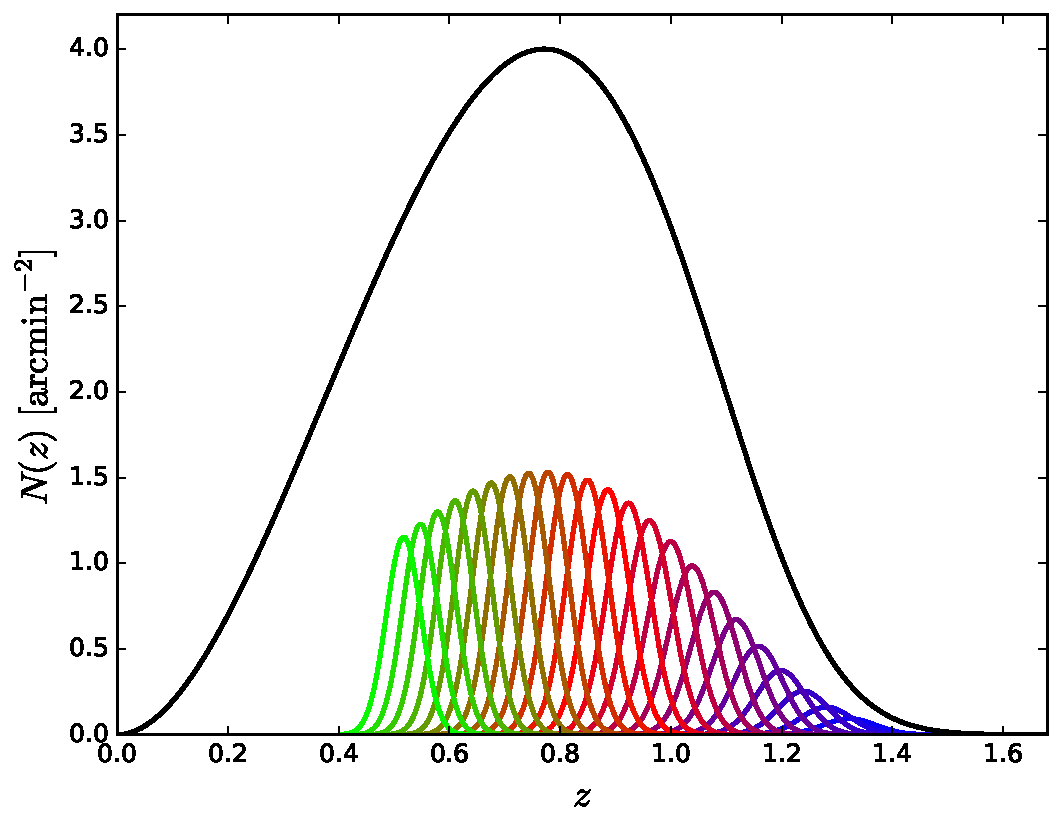
\includegraphics[width=0.49\textwidth]{Figs/nz_lsst_gc}
      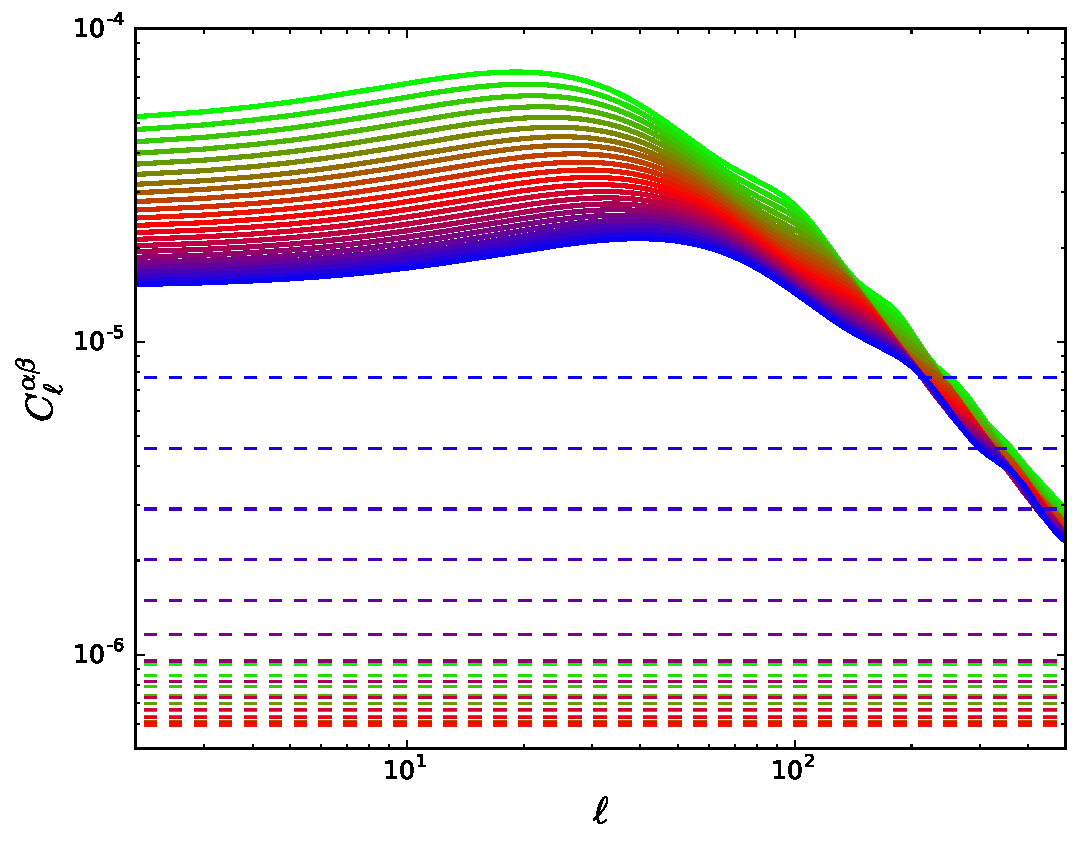
\includegraphics[width=0.49\textwidth]{Figs/c_ij_gc}
      \caption{{\sl Left}: redshift distribution and bins considered for the K-L analysis of a strawman large-scale-structure survey targeting a sample of red galaxies. {\sl Right}: clustering auto-power spectra of the redshift bins shown in the left panel. The signal and noise power spectra are shown as thick solid and thin dashed lines respectively.}\label{fig:nz_gc}
    \end{figure*}
    \begin{figure}
      \centering
      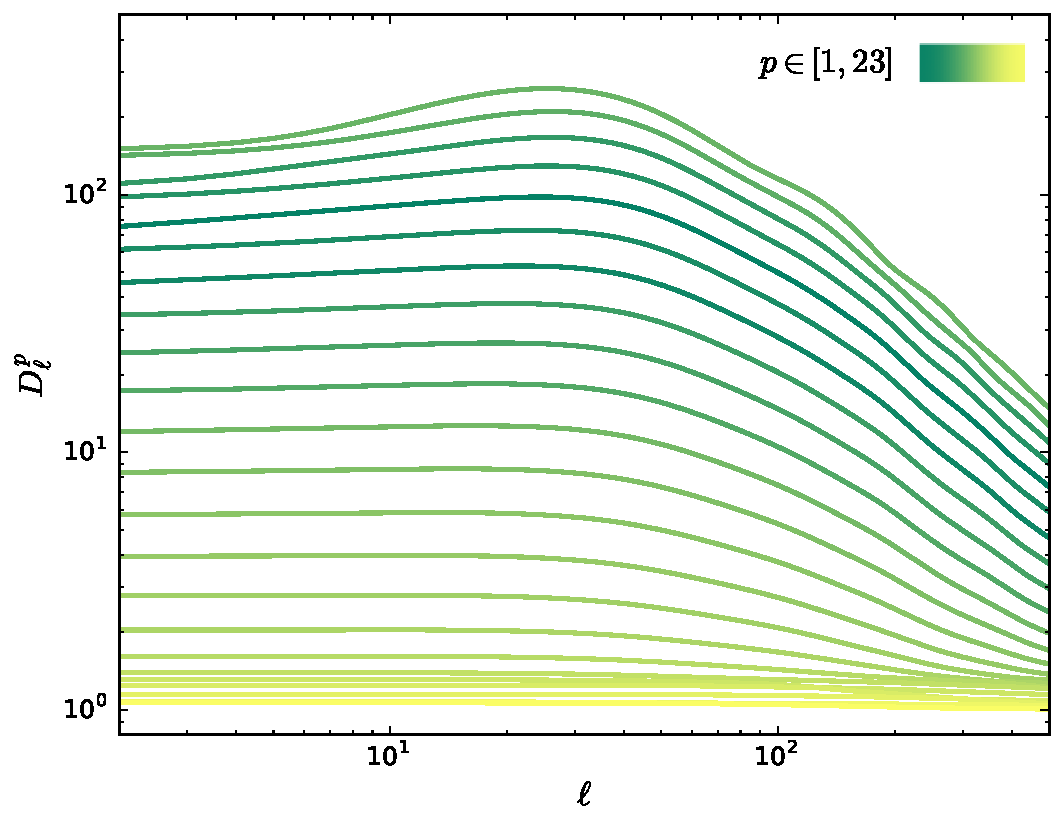
\includegraphics[width=0.49\textwidth]{Figs/d_p_gc}
      \caption{Power spectra of the K-L eigenmodes for the strawman weak large-scale-structure survey. Unlike in the case of weak lensing, a large number of eigenmodes are signal-dominated. This is due to the overall higher signal-to-noise ratio of galaxy clustering with respect to galaxy shear as well as to the smaller correlations between distant bins.}\label{fig:dp_gc}
    \end{figure}
    \begin{figure*}
      \centering
      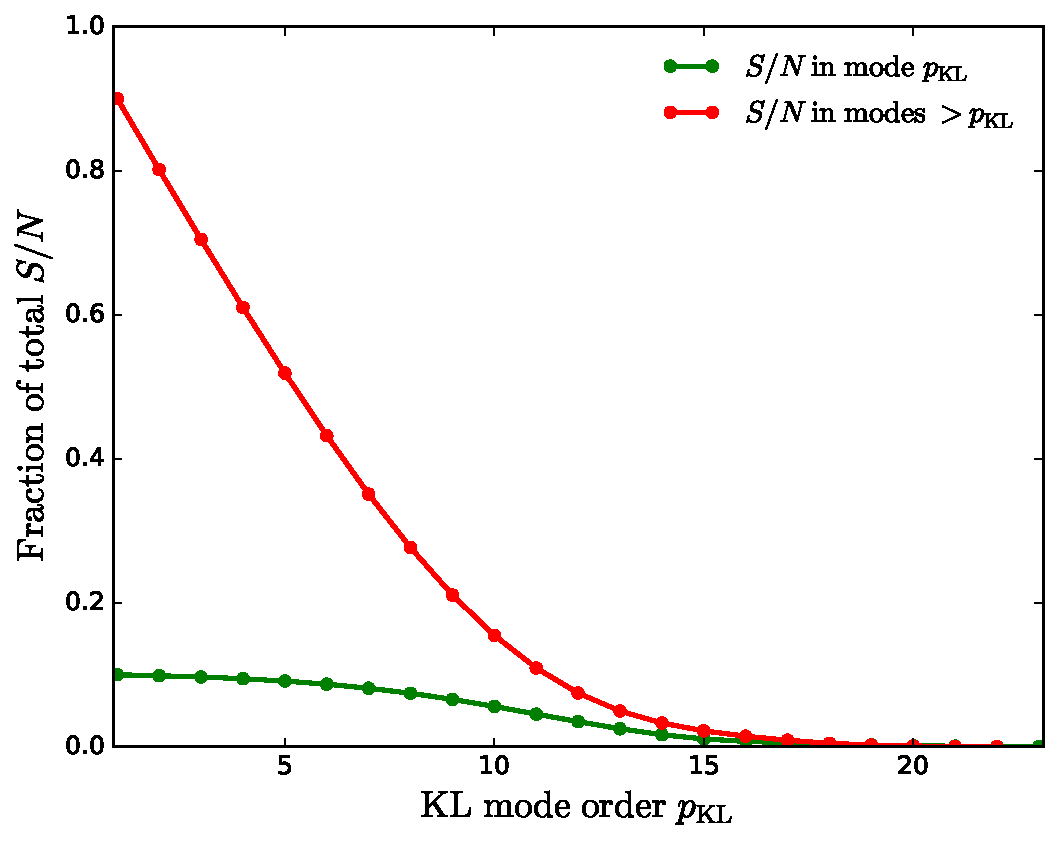
\includegraphics[width=0.49\textwidth]{Figs/information_gc}
      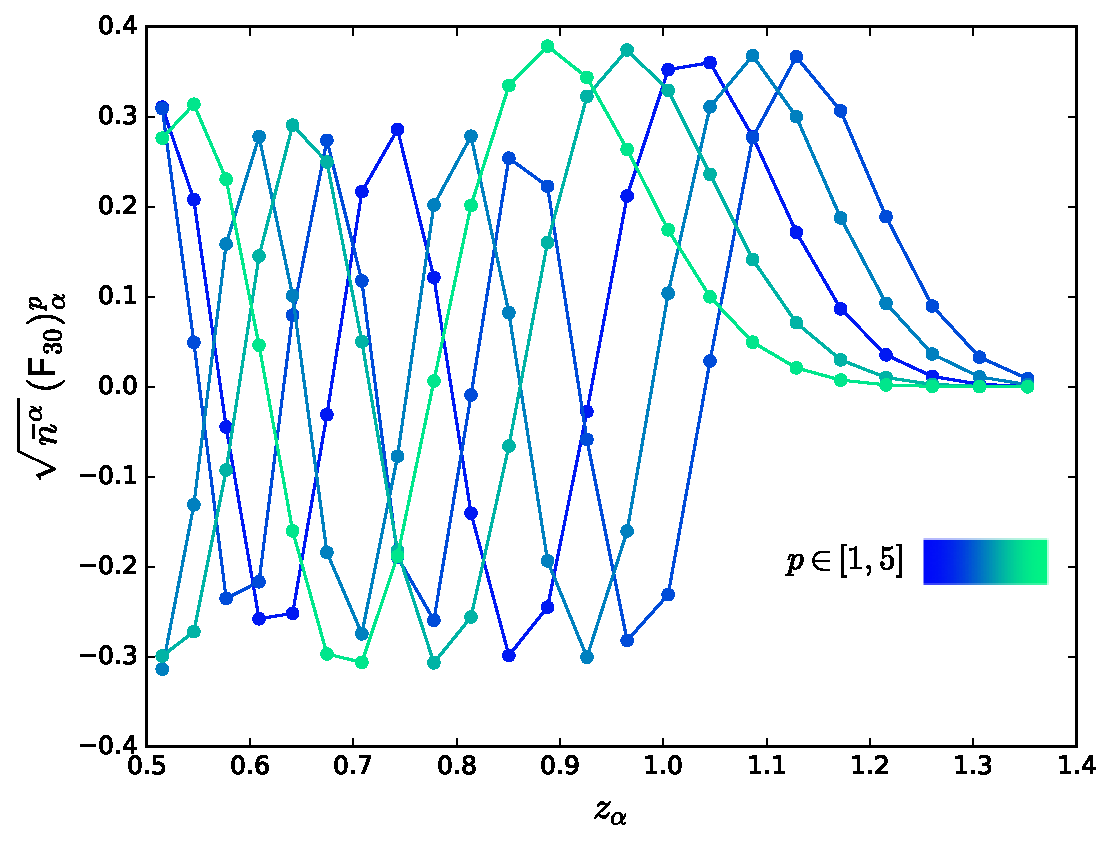
\includegraphics[width=0.49\textwidth]{Figs/kl_modes_gc}
      \caption{{\sl Left}: information content of the different K-L eigenmodes for the strawman galaxy clustering survey. The bulk of the information ($>90\%$) on $f_{\rm NL}$ is encoded in the first 12 modes. {\sl Left}: the first 5 K-L modes for $\ell=30$. The sinusoidal shape of the modes agrees with the expectation that, in the limit of $\sigma_z\rightarrow0$ and no background redshift dependence, the K-L modes should be given by the spherical Bessel functions. }\label{fig:kl_gc}
    \end{figure*}
    It is expected that future large-scale photometric surveys will make the search for primordial non-Gaussianity one of the main science cases. This can be achieved throught the excess power a non-zero value of $f_{\rm NL}$ generates in the two-point statistics of biased tracers of the matter distribution on large scales CITES. Since the signal is most relevant on large scales, one can expect most of the information on $f_{\rm NL}$ to be concentrated in a small number of radial modes, which makes the K-L decomposition described above an ideal analysis method.
    
    To explore this possibility we have considered a strawman photometric survey targeting a sample of red galaxies, characterized by their higher bias and better photo-$z$ uncertainties than their blue counterparts.The sample we consider is compatible with what could be observed by LSST, characterized by the redshift distribution shown in the left panel of Fig. \ref{fig:nz_gc} (full details can be found in CITE). We assume a photo-$z$ uncertainty of $\sigma_z=0.02\,(1+z)$ and split the sample into redshift bins in photo-$z$ space with $z_{\rm ph}>0.5$ and a width given by the photo-$z$ uncertainty at the bin centre. The resulting set of 23 bins is shown in the left panel of Fig. \ref{fig:nz_gc}. In the case of galaxy clustering, the transfer functions entering the signal power spectrum (see Eq. \ref{eq:cl_generic} are given by:
%    \begin{widetext}
    \begin{align}\nonumber
      &\Delta^{\delta,\alpha}_\ell(k)\equiv\int dz\,\phi^\alpha(z)\,\Psi_\ell(k,z)\,\sqrt{P(k,z)},\\\label{eq:tgc_dr}
      &\Psi_\ell(k,z)=b^\alpha(z)j_\ell(k\,\chi(z))-f(z)j_\ell''(k\,\chi(z))
    \end{align}
%    \end{widetext}
    where $b^\alpha(z)$ is the galaxy bias and $f(z)\equiv d\log\delta/d\log a$ is the growth rate of structure (we have kept the contribution from redshift-space distortions at linear order but ignored the effect of magnification bias). The auto-power spectra for our set of 23 bins are shown in the right panel of Fig. \ref{fig:nz_gc}.
    
    Using the prescription described in Section \ref{ssec:method.klbasis}, we find the K-L eigenmodes and associated power spectra, and rank them according to their contribution to the total Fisher matrix element of $f_{\rm NL}$. The power spectra of the K-L modes are shown in Figure \ref{fig:dp_gc}. Unlike the case of weak lensing, the information encoded in the galaxy overdensity is local in redshift (as opposed to integrated). Thus the correlation between different bins decays rapidly with redshift separation, and we find a much larger number of signal-dominated modes (e.g. compare with the analogous figure for weak lensing, Fig. \ref{fig:dp_wl}). The information on $f_{\rm NL}$ contained in each mode is shown in the left panel of Fig. \ref{fig:kl_gc}. In this case, the information is evenly spread across the first $\sim10$ modes, and 90\% of the total constraining power can be achieved by considering the first 12 eigenvectors. The form of the first 5 of these eigenvectors for $\ell=30$ are shown in the right panel of Fig. \ref{fig:kl_gc}. The eigenmodes are sinusoids with varying frequencies, in agreement with the expectation that, in the limit of $\sigma_z\rightarrow0$ and no background redshift dependence, the K-L decomposition is achieved by the spherical Bessel functions (see Section \ref{ssec:results.bessel}).
    
  \subsection{Correlated contaminants} \label{ssec:results.cc}
    \subsubsection{Intrinsic alignments} \label{sssec:results.cc.ia}
      Contamination of the weak lensing signal by locally correlated galaxy shapes, commonly known as ``intrinsic alignments'' (IA), is one of the main concerns for shear surveys. This contaminant cannot be described as an uncorrelated source of irreducible noise, since the causes of IA (e.g. the local tidal field in the non-linear alignment model CITE) are likely correlated the lensing potential.
      
      The K-L decomposition, as described in Section \ref{sssec:method.klbasis.cr}, can therefore be used to design an optimal basis that maximizes the true lensing signal over any correlated component. The method is similar to the so-called ``nulling'' approach of CITE.     
      
    \subsubsection{Magnification bias} \label{sssec:results.cc.mb}
      Gravitational lensing of the galaxy positions alters the clustering pattern of galaxies through the so-called magnification bias effect. This appears as an extra term in the galaxy clustering transfer function (Eq. \ref{eq:tgc_dr}):
      \begin{align}\nonumber
        &\Delta^{M,\alpha}_\ell(k)=-2\ell(\ell+1)\int\,d\chi W^{M,\alpha}(\chi)\frac{j_\ell(k\chi)}{k^2a(\chi)}\sqrt{P(k,z(\chi))},\\
        &W^{M,\alpha}(\chi)=\frac{3H_0^2\Omega_M}{2}\int_{z(\chi)}^\infty dz'\,\phi^\alpha(z')\frac{2-5\,s}{2}\,\frac{\chi(z')-\chi}{\chi(z')\chi},
      \end{align}
      where $s$ is the tilt in the number counts of sources as a function of magnitude limit.
      
      With the aim of measuring this effect, one can think of the density and RSD terms as correlated contaminants on top of it (i.e. taking the place of intrinsic alignments in the case of shear measurements), and thus develop an optimal K-L eigenbasis to measure it CITE.

    
\section{Practical example: weak lensing}
  \lipsum[2]

\section{Discussion}\label{sec:discussion}
  \lipsum[3]

\section*{Acknowledgements}
  \lipsum[4]
  
\bibliography{paper}

\appendix
\onecolumngrid
\section{Pseudo-$C_\ell$ estimation of the K-L modes}\label{app:pcl}
  One of the standard methods to estimate the angular power spectrum of any two quantities in the cut sky is the so-called pseudo-$C_\ell$ estimator. This section adapts this method to the modes resulting from the K-L decomposition described before.
  
  The standard pseudo-$C_\ell$ method is based on computing the spherical harmonic coefficients of the mask field:
  \begin{equation}
    \tilde{a}^\alpha_{\ell m}=\int d\nv\,a^\alpha(\nv)\,w^\alpha(\nv),
  \end{equation}
  where $w^\alpha$ is the weights map characterizing the mask of the field $a^\alpha$. One then estimates the power spectrum of this object by averaging over $m$ for each $\ell$:
  \begin{equation}
    \tilde{C}^{\alpha\beta}_\ell\equiv\frac{\sum_m\tilde{a}^\alpha_{\ell m}\tilde{a}^{\beta *}_{\ell m}}{2\ell+1}.
  \end{equation}
  This object is then related to the true underlying power spectrum through a mode-coupling matrix $M^{\alpha\beta}_{\ell\ell'}$ such that
  \begin{equation}
    \tilde{C}^{\alpha\beta}_\ell=\sum_{\ell'}M^{\alpha\beta}_{\ell\ell'}C^{\alpha\beta}_{\ell'},\hspace{12pt}
    M^{\alpha\beta}_{\ell \ell'}\equiv\sum_{\ell''}\frac{(2\ell'+1)(2\ell''+1)}{4\pi}W^{\alpha\beta}_{\ell''}
    \left(
    \begin{array}{ccc}
      \ell & \ell' & \ell''\\
      0 & 0 & 0
    \end{array}
    \right)^2
  \end{equation}
  where the coupling matrix $M$ depends solely on the power spectrum of the masks $W^{\alpha\beta}_\ell\equiv(2\ell+1)^{-1}\sum_mw^\alpha_{\ell m}w^{\beta *}_{\ell m}$.
  
  The extension of this estimator to the power spectrum of the K-L modes is straightforward: we project the masked harmonic coefficients $\tilde{a}^\alpha$ over the K-L eigenvectors ${\sf E}$ (i.e. $\tilde{\bf b}_{\ell m}\equiv {\sf E}_\ell\circ\tilde{\bf a}_{\ell m}$) and compute their power spectra by averaging over $m$. The resulting estimator takes the form $\tilde{D}^p_\ell=\sum_{\ell'}M_{\ell\ell'}^{pp'}D^{p'}_{\ell'}$, where the new mode-coupling matrix is given by:
  \begin{equation}
    M^{pp'}_{\ell\ell'}\equiv M^{\alpha\beta}_{\ell\ell'}\left[({\sf E}_\ell)^p_\alpha({\sf N}^{-1})_{\alpha\alpha'}({\sf E}_{\ell'})^{p'}_{\alpha'}\right]\left[({\sf E}_\ell)^p_\beta({\sf N}^{-1})_{\beta\beta'}({\sf E}_{\ell'})^{p'}_{\beta'}\right]
    =M_{\ell\ell'}\left[({\sf E}_\ell)^p_\alpha({\sf N}^{-1}_\ell)_{\alpha\beta}({\sf E}_{\ell'})^{p'}_\beta\right]^2
  \end{equation}
  where the second equality holds only if all the maps $a^\alpha_\ell$ share the same mask $w$.\footnote{Note that, for full-sky coverage $M_{\ell\ell'}=\delta_{\ell\ell'}$ and using the orthonormality of ${\sf E}$ we get $M^{pp'}_{\ell\ell'}=\delta_{\ell\ell'}\delta_{pp'}$.}

\end{document}
